\chapter{Gradient Descent}
\label{chap:gradient_descent}

% ========================================
% SECTION 1: INTRODUCTION
% ========================================
\section{Introduction: Why Not Always Use OLS?}
In Chapter 3, we derived the Normal Equation:
$$ \boldsymbol{\beta} = (\mathbf{X}^T \mathbf{X})^{-1} \mathbf{X}^T \mathbf{Y} $$
This is a closed-form solution that gives the exact answer in one step. So why do we need another method?

\textbf{The Problem}: Inverting a matrix has a time complexity of $O(n^3)$.
\begin{itemize}
    \item If $n$ (number of features) is 10-100, OLS is super fast.
    \item If $n$ is 100,000 (common in NLP or image data), $O(n^3)$ becomes computationally impossible.
\end{itemize}

\begin{definition}
\textbf{Gradient Descent}: An iterative optimization algorithm that finds the minimum of a function by repeatedly taking steps in the direction opposite to the gradient (slope).
\end{definition}

% ========================================
% SECTION 2: INTUITION
% ========================================
\section{Intuition: The Blindfolded Hiker}
Imagine you are standing on a mountain, blindfolded. Your goal is to reach the bottom of the valley (the lowest point).
\begin{enumerate}
    \item \textbf{Feel the ground}: Determine which direction is downhill (the slope).
    \item \textbf{Take a step}: Move in that direction.
    \item \textbf{Repeat}: Keep doing this until the ground beneath you is flat (slope $\approx 0$).
\end{enumerate}

\textbf{The Loss Function is a Bowl}: For Linear Regression using MSE, the loss function $J(m, c)$ is \textbf{Convex} (bowl-shaped). It has only \textbf{one} minimum (the Global Minimum), so Gradient Descent is \textbf{guaranteed} to find it.

\begin{figure}[htbp]
\centering
\includegraphics[width=0.6\textwidth]{../02-supervised/assets/gradient_descent_bowl.png}
\caption{The Convex Loss Surface. Gradient Descent rolls down to the bottom.}
\label{fig:gd_bowl}
\end{figure}

% ========================================
% SECTION 3: MATHEMATICAL FORMULATION
% ========================================
\section{The Algorithm (Step-by-Step)}
Let $J(m, c) = \frac{1}{n} \sum (y_i - (mx_i + c))^2$ be the MSE Loss.

\textbf{Step 1: Initialize Parameters}
\begin{itemize}
    \item Start with random values (e.g., $m=0, c=0$).
\end{itemize}

\textbf{Step 2: Calculate the Gradient}
The gradient tells us the direction of steepest ascent. We move in the \textit{opposite} direction.
\begin{align}
    \frac{\partial J}{\partial m} &= -\frac{2}{n} \sum_{i=1}^{n} x_i (y_i - (mx_i + c)) \\
    \frac{\partial J}{\partial c} &= -\frac{2}{n} \sum_{i=1}^{n} (y_i - (mx_i + c))
\end{align}

\textbf{Step 3: Update Parameters}
Move against the gradient, scaled by the \textbf{Learning Rate} ($\eta$ or $\alpha$).
\begin{align}
    m_{\text{new}} &= m_{\text{old}} - \eta \cdot \frac{\partial J}{\partial m} \\
    c_{\text{new}} &= c_{\text{old}} - \eta \cdot \frac{\partial J}{\partial c}
\end{align}

\textbf{Step 4: Repeat} until convergence or max epochs reached.

% ========================================
% SECTION 4: LEARNING RATE
% ========================================
\section{The Learning Rate ($\eta$)}
The learning rate is a crucial hyperparameter.
\begin{itemize}
    \item \textbf{Too Small}: Tiny steps. Convergence is very \textbf{slow}.
    \item \textbf{Too Large}: Giant jumps. Might \textbf{overshoot} the minima and diverge.
    \item \textbf{Just Right}: Converges smoothly and efficiently.
\end{itemize}

% ========================================
% SECTION 5: THE IMPORTANCE OF FEATURE SCALING
% ========================================
\section{The Importance of Feature Scaling}
\label{sec:gd_scaling}

You might have noticed that in our Scikit-Learn example, we used `StandardScaler`. This is not optional for Gradient Descent; it is \textbf{mandatory}.

\subsection{The "Elongated Bowl" Problem}
Imagine predicting House Price using two features:
\begin{itemize}
    \item $x_1$: Number of Rooms (Range: 1 to 5).
    \item $x_2$: Area in sq ft (Range: 500 to 5000).
\end{itemize}

Since $x_2$ is 1000 times larger than $x_1$, a small change in its weight ($\beta_2$) will cause a massive explosion in the prediction ($y = \beta_1 x_1 + \beta_2 x_2$).
\begin{enumerate}
    \item The Loss Function becomes an **Elongated Bowl** (like a narrow taco shell).
    \item The Gradient will be very steep in one direction and very flat in the other.
    \item Gradient Descent will zig-zag wildly across the steep walls and take forever to reach the bottom.
\end{enumerate}

\subsection{The Solution: Scale Features}
When we scale both features to the same range (e.g., Mean=0, Variance=1):
\begin{enumerate}
    \item The Loss Function becomes a **Perfectly Round Bowl**.
    \item The Gradient points directly to the center.
    \item Convergence is straight and fast.
\end{enumerate}

\begin{figure}[htbp]
\centering
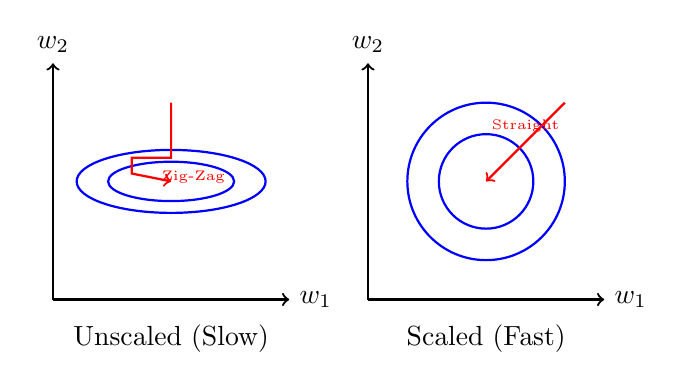
\begin{tikzpicture}
    % Unscaled (Elongated)
    \begin{scope}
        \draw[thick, ->] (0,0) -- (3,0) node[right] {$w_1$};
        \draw[thick, ->] (0,0) -- (0,3) node[above] {$w_2$};
        \draw[blue, thick] (1.5,1.5) ellipse (1.2cm and 0.4cm);
        \draw[blue, thick] (1.5,1.5) ellipse (0.8cm and 0.25cm);
        \draw[red, thick, ->] (1.5, 2.5) -- (1.5, 1.8) -- (1.0, 1.8) -- (1.0, 1.6) -- node[right, font=\tiny]{Zig-Zag} (1.5, 1.5);
        \node[below] at (1.5, -0.2) {Unscaled (Slow)};
    \end{scope}
    
    % Scaled (Round)
    \begin{scope}[xshift=4cm]
        \draw[thick, ->] (0,0) -- (3,0) node[right] {$w_1$};
        \draw[thick, ->] (0,0) -- (0,3) node[above] {$w_2$};
        \draw[blue, thick] (1.5,1.5) circle (1.0cm);
        \draw[blue, thick] (1.5,1.5) circle (0.6cm);
        \draw[red, thick, ->] (2.5, 2.5) -- node[above, font=\tiny]{Straight} (1.5, 1.5);
        \node[below] at (1.5, -0.2) {Scaled (Fast)};
    \end{scope}
\end{tikzpicture}
\caption{Feature Scaling transforms the Loss Surface from an elongated valley (slow zig-zag) to a round bowl (fast straight path).}
\label{fig:scaling_geometry}
\end{figure}

% ========================================
% SECTION 6: TYPES OF GRADIENT DESCENT
% ========================================
\section{Types of Gradient Descent}
How many data points do we use to calculate the gradient in one step?

\subsection{1. Batch Gradient Descent}
\begin{definition}
\textbf{Batch Gradient Descent}: Uses \textbf{ALL} $n$ data points to calculate the gradient for a single weight update.
\end{definition}

\textbf{Vectorized Gradient Formula}:
\begin{equation}
    \frac{\partial J}{\partial \boldsymbol{\beta}} = -\frac{2}{n} \mathbf{X}^T (\mathbf{Y} - \hat{\mathbf{Y}})
\end{equation}

\textbf{Update Rule}:
\begin{equation}
    \boldsymbol{\beta}_{\text{new}} = \boldsymbol{\beta}_{\text{old}} - \eta \cdot \left( -\frac{2}{n} \mathbf{X}^T (\mathbf{Y} - \hat{\mathbf{Y}}) \right)
\end{equation}

\textbf{Pros}: Stable convergence, accurate gradient.
\textbf{Cons}: Very slow for large datasets. Requires all data in RAM.

\begin{lstlisting}[language=Python, caption=Batch Gradient Descent from Scratch]
import numpy as np

class BatchGDRegressor:
    def __init__(self, learning_rate=0.01, epochs=100):
        self.lr = learning_rate
        self.epochs = epochs
        self.coef_ = None
        self.intercept_ = None
        
    def fit(self, X, y):
        n = X.shape[0]
        self.intercept_ = 0
        self.coef_ = np.ones(X.shape[1])
        
        for _ in range(self.epochs):
            # Vectorized prediction
            y_hat = np.dot(X, self.coef_) + self.intercept_
            
            # Vectorized gradients (ALL data)
            intercept_grad = -2 * np.mean(y - y_hat)
            coef_grad = -2 * np.dot(X.T, (y - y_hat)) / n
            
            # Update
            self.intercept_ -= self.lr * intercept_grad
            self.coef_ -= self.lr * coef_grad
\end{lstlisting}

\subsection{2. Stochastic Gradient Descent (SGD)}
\begin{definition}
\textbf{Stochastic Gradient Descent}: Uses \textbf{ONE} random data point to calculate the gradient and update weights.
\end{definition}

\textbf{Gradient for Single Point $i$}:
\begin{align}
    \frac{\partial J}{\partial \beta_0} &= -2 (y_i - \hat{y}_i) \\
    \frac{\partial J}{\partial \beta_j} &= -2 (y_i - \hat{y}_i) x_{ij}
\end{align}

\textbf{Pros}: Extremely fast iterations. Works for massive datasets (streaming).

\textbf{Cons}: Noisy convergence (zig-zag path). Might never settle exactly at minima.

\textbf{Solution: Learning Rate Decay}
\begin{equation}
    \eta_t = \frac{\eta_0}{1 + \text{decay} \times t}
\end{equation}
Start with a large learning rate to move fast, then decrease to settle precisely.

\begin{lstlisting}[language=Python, caption=Stochastic Gradient Descent from Scratch]
class SGDRegressor:
    def __init__(self, learning_rate=0.01, epochs=100):
        self.lr = learning_rate
        self.epochs = epochs
        
    def fit(self, X, y):
        n = X.shape[0]
        self.intercept_ = 0
        self.coef_ = np.ones(X.shape[1])
        
        for epoch in range(self.epochs):
            for _ in range(n):
                # Pick ONE random sample
                idx = np.random.randint(0, n)
                x_i, y_i = X[idx], y[idx]
                
                # Prediction for single row
                y_hat = np.dot(x_i, self.coef_) + self.intercept_
                
                # Gradients (no summation)
                intercept_grad = -2 * (y_i - y_hat)
                coef_grad = -2 * (y_i - y_hat) * x_i
                
                # Update IMMEDIATELY
                self.intercept_ -= self.lr * intercept_grad
                self.coef_ -= self.lr * coef_grad
\end{lstlisting}

\begin{figure}[htbp]
\centering
\includegraphics[width=0.7\textwidth]{../02-supervised/assets/batch_vs_sgd_contour.png}
\caption{Batch GD (smooth path) vs SGD (noisy zig-zag path).}
\label{fig:batch_vs_sgd}
\end{figure}

\subsection{3. Mini-Batch Gradient Descent}
\begin{definition}
\textbf{Mini-Batch Gradient Descent}: Uses a small \textbf{batch} of $k$ data points (e.g., 32, 64) for each update. Best of both worlds.
\end{definition}

\textbf{Algorithm}:
\begin{enumerate}
    \item Decide batch size $k$ (e.g., 32).
    \item Shuffle data at start of each epoch.
    \item Loop through batches, compute gradient on each batch, update weights.
\end{enumerate}

\begin{lstlisting}[language=Python, caption=Mini-Batch Gradient Descent from Scratch]
class MiniBatchGDRegressor:
    def __init__(self, learning_rate=0.01, epochs=100, batch_size=32):
        self.lr = learning_rate
        self.epochs = epochs
        self.batch_size = batch_size
        
    def fit(self, X, y):
        n = X.shape[0]
        self.intercept_ = 0
        self.coef_ = np.ones(X.shape[1])
        num_batches = n // self.batch_size
        
        for epoch in range(self.epochs):
            # Shuffle data
            indices = np.random.permutation(n)
            X_shuffled, y_shuffled = X[indices], y[indices]
            
            for j in range(num_batches):
                start = j * self.batch_size
                end = start + self.batch_size
                X_batch = X_shuffled[start:end]
                y_batch = y_shuffled[start:end]
                
                # Vectorized on batch
                y_hat = np.dot(X_batch, self.coef_) + self.intercept_
                intercept_grad = -2 * np.mean(y_batch - y_hat)
                coef_grad = -2 * np.dot(X_batch.T, (y_batch - y_hat)) / self.batch_size
                
                self.intercept_ -= self.lr * intercept_grad
                self.coef_ -= self.lr * coef_grad
\end{lstlisting}

\begin{figure}[htbp]
\centering
\includegraphics[width=0.8\textwidth]{../02-supervised/assets/gd_variants_comparison.png}
\caption{Comparison of all three GD variants. Mini-Batch is the practical choice.}
\label{fig:gd_variants}
\end{figure}

\subsection{Comparison Table}
\begin{center}
\begin{tabular}{|l|c|c|c|}
\hline
\textbf{Feature} & \textbf{Batch GD} & \textbf{SGD} & \textbf{Mini-Batch GD} \\ \hline
Data per Update & All $n$ & 1 & $k$ (e.g., 32) \\ \hline
Speed per Update & Slow & Very Fast & Fast \\ \hline
Updates per Epoch & 1 & $n$ & $n/k$ \\ \hline
Convergence & Smooth & Noisy & Slightly wavy \\ \hline
Memory & High & Low & Medium \\ \hline
\end{tabular}
\end{center}

% ========================================
% SECTION 6: CONVEX VS NON-CONVEX
% ========================================
\section{Convex vs Non-Convex Functions}
\begin{itemize}
    \item \textbf{Convex Function}: Like a bowl. Has only \textbf{one} Global Minimum. GD is guaranteed to find it.
    \item \textbf{Non-Convex Function}: Like a rocky terrain. Has multiple \textbf{Local Minima} and \textbf{Saddle Points}. GD might get stuck.
\end{itemize}

\begin{figure}[htbp]
\centering
\includegraphics[width=0.7\textwidth]{../02-supervised/assets/convex_vs_non_convex.png}
\caption{Convex (guaranteed global) vs Non-Convex (can get stuck).}
\label{fig:convex_nonconvex}
\end{figure}

% ========================================
% SECTION 7: SCIKIT-LEARN
% ========================================
\section{Scikit-Learn Implementation}
\begin{lstlisting}[language=Python, caption=SGDRegressor in Scikit-Learn]
from sklearn.linear_model import SGDRegressor
from sklearn.preprocessing import StandardScaler
from sklearn.pipeline import make_pipeline

# Always scale features for GD-based methods!
model = make_pipeline(
    StandardScaler(),
    SGDRegressor(max_iter=1000, tol=1e-3, eta0=0.01)
)
model.fit(X_train, y_train)
print(f"Score: {model.score(X_test, y_test):.3f}")
\end{lstlisting}

% ========================================
% SECTION 8: HOTS QUESTIONS
% ========================================
\section{HOTS: Interview Questions}
\textbf{Q1: What is the difference between Local Minima and Global Minima?}
\begin{itemize}
    \item \textbf{Global Minima}: The absolute lowest point of the entire function.
    \item \textbf{Local Minima}: A point lower than its immediate neighbors, but not the absolute lowest.
    \item For Linear Regression (Convex Loss), there is only one minimum, so Local = Global.
\end{itemize}

\textbf{Q2: Why is SGD faster than Batch GD even though it is "noisier"?}
\begin{itemize}
    \item SGD makes $n$ updates per epoch (one per sample).
    \item Batch GD makes only 1 update per epoch.
    \item SGD converges in fewer epochs despite the noise.
\end{itemize}

\textbf{Q3: Why do we shuffle data in Mini-Batch GD?}
\begin{itemize}
    \item To avoid learning patterns from the order of data.
    \item If data is sorted by class, each batch would be homogeneous, leading to poor gradients.
\end{itemize}

\textbf{Q4: What is a Saddle Point?}
\begin{itemize}
    \item A point where the gradient is zero, but it is neither a minimum nor a maximum.
    \item The surface curves upward in one direction and downward in another.
    \item GD can get stuck here in non-convex problems (like Neural Networks).
\end{itemize}

% ========================================
% SECTION 9: QUICK REFERENCE
% ========================================
\section{Quick Reference Card}

\begin{center}
\fbox{\parbox{0.9\textwidth}{
\textbf{GRADIENT DESCENT - CHEAT SHEET}
\vspace{0.3cm}

\textbf{Core Update Rule}: $\theta := \theta - \alpha \cdot \nabla J(\theta)$

\textbf{Variants Comparison}:
\begin{center}
\begin{tabular}{|l|c|c|c|}
\hline
& \textbf{Batch} & \textbf{SGD} & \textbf{Mini-Batch} \\ \hline
Data/Update & All $n$ & 1 & $k$ (32/64) \\ \hline
Speed & Slow & Fast & Balanced \\ \hline
Noise & None & High & Low \\ \hline
\end{tabular}
\end{center}

\textbf{Learning Rate ($\alpha$)}:
\begin{itemize}
    \item Too high $\rightarrow$ Overshoots, diverges
    \item Too low $\rightarrow$ Converges slowly
    \item Start: 0.01 or 0.001
\end{itemize}

\textbf{CRITICAL}: Always scale features before GD! (Elongated Bowl Problem)

\textbf{Scikit-Learn}: \texttt{SGDRegressor(eta0=0.01, max\_iter=1000)}

\textbf{Interview Gold}:
\begin{itemize}
    \item Batch GD = 1 update/epoch; SGD = $n$ updates/epoch
    \item Convex = guaranteed global min; Non-convex = may get stuck
    \item Saddle point: gradient = 0, but not a minimum
\end{itemize}
}}
